% LaTeX .tex example for the proceedings of
% CLIV 3 - III Latin American Wind Engineering Congress
% November, 5-8, 2018, São Paulo, SP, Brazil
%
% Based on the template of the proceedings of COBEM2017 
% MODELO CLIV 3

\documentclass[10pt,fleqn,a4paper,twoside]{article}
\usepackage{cliv}
\usepackage[utf8]{inputenc}
\usepackage[english,portuguese,spanish]{babel}
\def\shortauthor{P. Jabardo, L. Alves, G. Borelli and G. Nader}
\def\shorttitle{Anemômetro de Baixo Custo para Ensaios de Conforto}

\begin{document}
	\fphead
\hspace*{-2.5mm}\begin{tabular}{||p{\textwidth}}
\begin{center}
\vspace{-4mm}
\title{ %CLIV3-2018-XXXX\\
ANEMÔMETRO DE BAIXO CUSTO PARA ENSAIOS DE CONFORTO} % (XXXX is the manuscript number)
\end{center}
                  
\authors{Paulo José Saiz Jabardo} \\
\authors{Leandro Alves} \\
\authors{Gabriel Borelli}\\                  
\authors{Gilder Nader}\\
\institution{Instituto de Pesquisas Tecnológicas - Av. Prof. Almeida Prado 532, São Paulo, SP}\\
\institution{pjabardo@ipt.br, leoalvs@ipt.br, gborelli@ipt.br, gnader@ipt.br} \\
\\
\abstract{\textbf{Abstract.} Um anemômetro de baixo custo e fácil construção é descrito. Este anemômetro utiliza como um termistor aquecido como sensor e microcontroladores disponíveis no mercado. Operação em corrente constante ou temperatura constante são analisados.}\\
\\
\keywords{\textbf{Keywords:} anemômetro, túnel de vento, corrente constante, temperatura constante}\\
\end{tabular}

\section{INTRODUÇÃO}

Medição de velocidade é um dos aspectos mais importantes em qualquer túnel de vento. Diversos tipos de sensores existem para diferentes aplicações. Em ensaios de conforte de pedestres existe a necessidade de medir velocidade baixas em pontos próximos ao chão com vento vindo de qualquer direção. O sensor de Irwin \citep{Irwin81} tem sido muito utilizado mas pode apresentar algumas dificuldades. Talvez a maior dificuldade seja o diferencial de pressão baixo resultante das baixas velocidades próximas ao chão e coeficiente de pressão baixo o que aumenta consideravelmente a incerteza de medição. A própria geometria do sensor impede que seja utilizado para medir a ventilação em janelas por exemplo. Mesmo sendo simples, a construção dos sensores de Irwin requer de usinagem de precisão e sua instalação pode ser difícil em algumas situações. Neste trabalho, um sensor de velocidade de baixo custo é proposto que resolve algumas destas dificuldades.

Termoanemômetros são muito comuns tanto na indústria quanto na academia. Até hoje, o anemômetro de fio quente é a espinha dorsal no que se refere à medição de turbulência. Os sensores de fio quente são caros e frágeis e termoanemômetros industriais, além de caros (quando se deseja medir diversos velocidades simultaneamente) são em geral grandes demais para serem colocados dentro de uma maquete de uma área construída. Mas o princípio tem algumas vantangens. Ao contrário do sensor de Irwin, no qual a pressão varia com o quadrado da velocidade, a resposta de um termoanemômetro varia, aproximadamente com a raíz quadrada da velocidade, de modo que para velocidades mais baixas, o anemômetro é mais sensível: neste caso a não linearidade do sensor ajuda nas medições próximas ao chão.

Termistores são elementos semicondutores cuja resistência varia de maneira significativa com a temperatura, em particular os termistores com coeficiente de temperatura negativa (NTC), cuja resistência diminui com o aumento da temperatura, são componentes de baixo custo, com pequenas dimensões e robustos. A figura \ref{fig:termistor} mostra uma foto de um termistor. Este termistor apresenta uma geometria esférica com diâmetro aproximado de 2 mm.

\begin{figure}[h!]
\centering
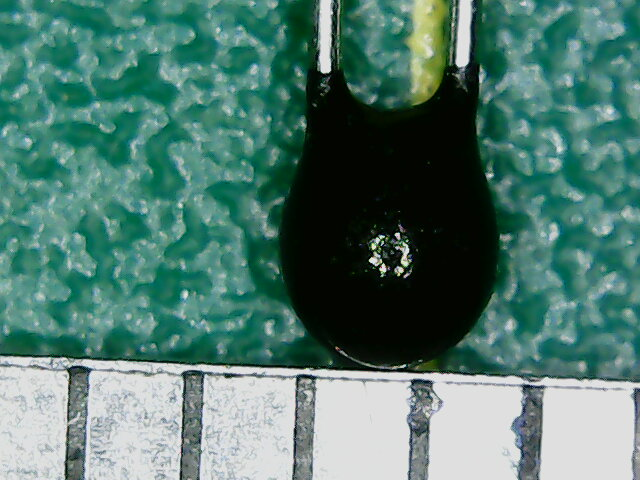
\includegraphics[width=0.5\textwidth]{../../figures/termistor.jpg}
\caption{Foto de um termistor com diâmetro aproximado de 2 mm}
\label{fig:termistor}
\end{figure}

Neste artigo, o comportamento do termistor como sensor de velocidade será modelado procurando mostrar a viabilidade do mesmo em estudos de conforto de pedestre. Em seguida, dois circuitos eletrônicos são propostos para a medição de velocidades. O primeiro circuito, mais simples, utilizando o princípio de corrente constante é apresentado. O segundo circuito, utilizando o princío de temperatura constante é analisado em seguida.

\section{PRINCÍPIOS DE FUNCIONAMENTO DE TERMOANEMÔMETROS}

A perda de calor de um corpo aquecido varia com a velocidade: quanto maior a velocidade ao redor do corpo maior a perda de calor. Quando uma corrente elétrica circula por 

\section{ACKNOWLEDGEMENTS}
This optional section must be placed before the list of references.

\section{REFERENCES} 

The list of references must be introduced as a new section, located at the end of the paper. The first line of each reference must be aligned at left.  All the other lines must be indented by 0.5 cm from the left margin. All references included in the reference list must have been mentioned in the text.

References must be listed in alphabetical order, according to the last name of the first author. See the following examples:

\bibliographystyle{cliv}
\renewcommand{\refname}{}
%\bibliography{bibfile}
\bibliography{bibanem}
\section{RESPONSIBILITY NOTICE}

The following text, properly adapted to the number of authors, must be included in the last section of the paper:

The author(s) is (are) the only responsible for the printed material included in this paper.

\end{document}
